\documentclass[1p]{elsarticle_modified}
%\bibliographystyle{elsarticle-num}

%\usepackage[colorlinks]{hyperref}
%\usepackage{abbrmath_seonhwa} %\Abb, \Ascr, \Acal ,\Abf, \Afrak
\usepackage{amsfonts}
\usepackage{amssymb}
\usepackage{amsmath}
\usepackage{amsthm}
\usepackage{scalefnt}
\usepackage{amsbsy}
\usepackage{kotex}
\usepackage{caption}
\usepackage{subfig}
\usepackage{color}
\usepackage{graphicx}
\usepackage{xcolor} %% white, black, red, green, blue, cyan, magenta, yellow
\usepackage{float}
\usepackage{setspace}
\usepackage{hyperref}

\usepackage{tikz}
\usetikzlibrary{arrows}

\usepackage{multirow}
\usepackage{array} % fixed length table
\usepackage{hhline}

%%%%%%%%%%%%%%%%%%%%%
\makeatletter
\renewcommand*\env@matrix[1][\arraystretch]{%
	\edef\arraystretch{#1}%
	\hskip -\arraycolsep
	\let\@ifnextchar\new@ifnextchar
	\array{*\c@MaxMatrixCols c}}
\makeatother %https://tex.stackexchange.com/questions/14071/how-can-i-increase-the-line-spacing-in-a-matrix
%%%%%%%%%%%%%%%

\usepackage[normalem]{ulem}

\newcommand{\msout}[1]{\ifmmode\text{\sout{\ensuremath{#1}}}\else\sout{#1}\fi}
%SOURCE: \msout is \stkout macro in https://tex.stackexchange.com/questions/20609/strikeout-in-math-mode

\newcommand{\cancel}[1]{
	\ifmmode
	{\color{red}\msout{#1}}
	\else
	{\color{red}\sout{#1}}
	\fi
}

\newcommand{\add}[1]{
	{\color{blue}\uwave{#1}}
}

\newcommand{\replace}[2]{
	\ifmmode
	{\color{red}\msout{#1}}{\color{blue}\uwave{#2}}
	\else
	{\color{red}\sout{#1}}{\color{blue}\uwave{#2}}
	\fi
}

\newcommand{\Sol}{\mathcal{S}} %segment
\newcommand{\D}{D} %diagram
\newcommand{\A}{\mathcal{A}} %arc


%%%%%%%%%%%%%%%%%%%%%%%%%%%%%5 test

\def\sl{\operatorname{\textup{SL}}(2,\Cbb)}
\def\psl{\operatorname{\textup{PSL}}(2,\Cbb)}
\def\quan{\mkern 1mu \triangleright \mkern 1mu}

\theoremstyle{definition}
\newtheorem{thm}{Theorem}[section]
\newtheorem{prop}[thm]{Proposition}
\newtheorem{lem}[thm]{Lemma}
\newtheorem{ques}[thm]{Question}
\newtheorem{cor}[thm]{Corollary}
\newtheorem{defn}[thm]{Definition}
\newtheorem{exam}[thm]{Example}
\newtheorem{rmk}[thm]{Remark}
\newtheorem{alg}[thm]{Algorithm}

\newcommand{\I}{\sqrt{-1}}
\begin{document}

%\begin{frontmatter}
%
%\title{Boundary parabolic representations of knots up to 8 crossings}
%
%%% Group authors per affiliation:
%\author{Yunhi Cho} 
%\address{Department of Mathematics, University of Seoul, Seoul, Korea}
%\ead{yhcho@uos.ac.kr}
%
%
%\author{Seonhwa Kim} %\fnref{s_kim}}
%\address{Center for Geometry and Physics, Institute for Basic Science, Pohang, 37673, Korea}
%\ead{ryeona17@ibs.re.kr}
%
%\author{Hyuk Kim}
%\address{Department of Mathematical Sciences, Seoul National University, Seoul 08826, Korea}
%\ead{hyukkim@snu.ac.kr}
%
%\author{Seokbeom Yoon}
%\address{Department of Mathematical Sciences, Seoul National University, Seoul, 08826,  Korea}
%\ead{sbyoon15@snu.ac.kr}
%
%\begin{abstract}
%We find all boundary parabolic representation of knots up to 8 crossings.
%
%\end{abstract}
%\begin{keyword}
%    \MSC[2010] 57M25 
%\end{keyword}
%
%\end{frontmatter}

%\linenumbers
%\tableofcontents
%
\newcommand\colored[1]{\textcolor{white}{\rule[-0.35ex]{0.8em}{1.4ex}}\kern-0.8em\color{red} #1}%
%\newcommand\colored[1]{\textcolor{white}{ #1}\kern-2.17ex	\textcolor{white}{ #1}\kern-1.81ex	\textcolor{white}{ #1}\kern-2.15ex\color{red}#1	}

{\Large $\underline{12a_{1219}~(K12a_{1219})}$}

\setlength{\tabcolsep}{10pt}
\renewcommand{\arraystretch}{1.6}
\vspace{1cm}\begin{tabular}{m{100pt}>{\centering\arraybackslash}m{274pt}}
\multirow{5}{120pt}{
	\centering
	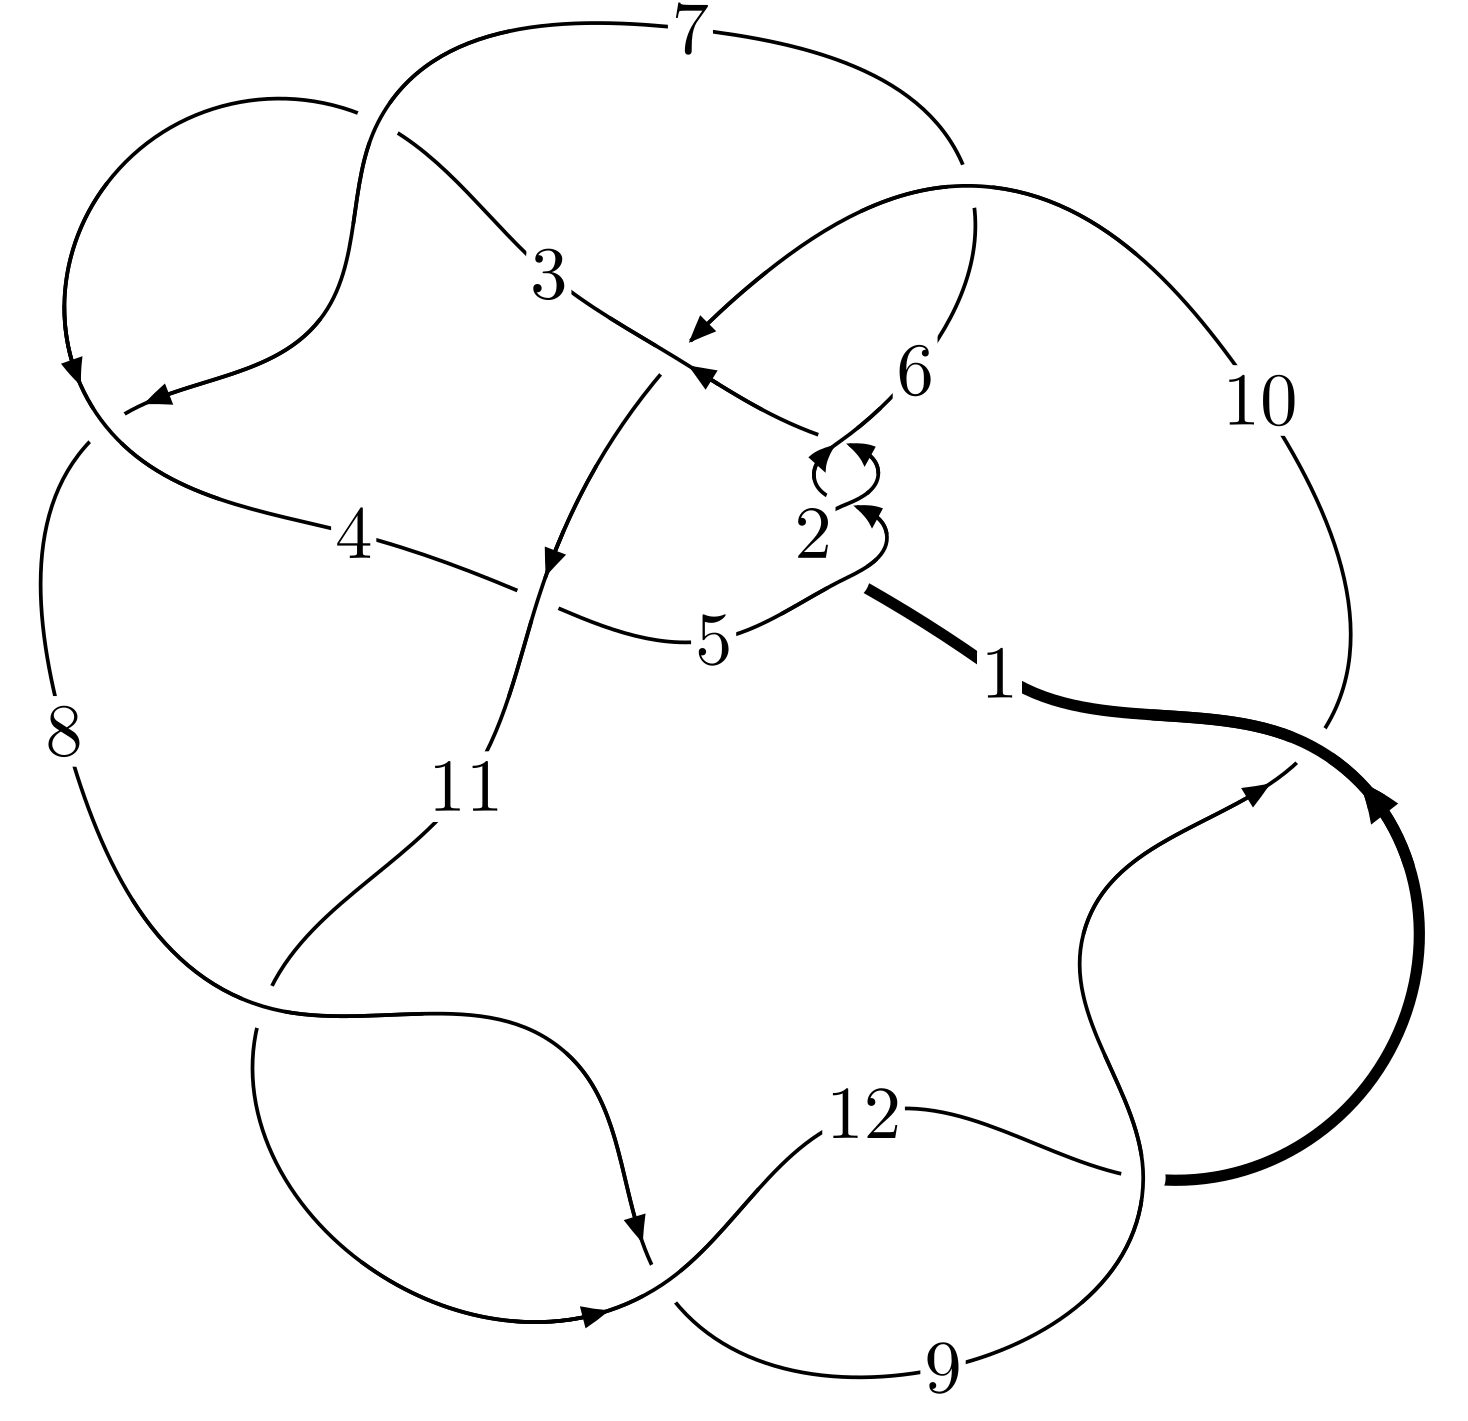
\includegraphics[width=112pt]{../../../GIT/diagram.site/Diagrams/png/2020_12a_1219.png}\\
\ \ \ A knot diagram\footnotemark}&
\allowdisplaybreaks
\textbf{Linearized knot diagam} \\
\cline{2-2}
 &
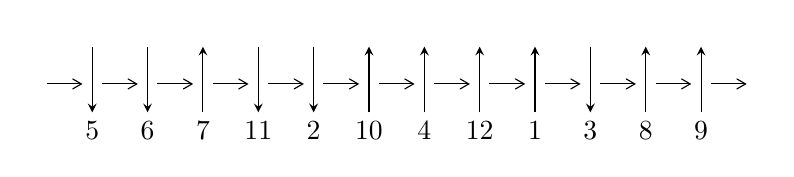
\begin{tikzpicture}[x=20pt, y=17pt]
	% nodes
	\node (C0) at (0, 0) {};
	\node (C1) at (1, 0) {};
	\node (C1U) at (1, +1) {};
	\node (C1D) at (1, -1) {5};

	\node (C2) at (2, 0) {};
	\node (C2U) at (2, +1) {};
	\node (C2D) at (2, -1) {6};

	\node (C3) at (3, 0) {};
	\node (C3U) at (3, +1) {};
	\node (C3D) at (3, -1) {7};

	\node (C4) at (4, 0) {};
	\node (C4U) at (4, +1) {};
	\node (C4D) at (4, -1) {11};

	\node (C5) at (5, 0) {};
	\node (C5U) at (5, +1) {};
	\node (C5D) at (5, -1) {2};

	\node (C6) at (6, 0) {};
	\node (C6U) at (6, +1) {};
	\node (C6D) at (6, -1) {10};

	\node (C7) at (7, 0) {};
	\node (C7U) at (7, +1) {};
	\node (C7D) at (7, -1) {4};

	\node (C8) at (8, 0) {};
	\node (C8U) at (8, +1) {};
	\node (C8D) at (8, -1) {12};

	\node (C9) at (9, 0) {};
	\node (C9U) at (9, +1) {};
	\node (C9D) at (9, -1) {1};

	\node (C10) at (10, 0) {};
	\node (C10U) at (10, +1) {};
	\node (C10D) at (10, -1) {3};

	\node (C11) at (11, 0) {};
	\node (C11U) at (11, +1) {};
	\node (C11D) at (11, -1) {8};

	\node (C12) at (12, 0) {};
	\node (C12U) at (12, +1) {};
	\node (C12D) at (12, -1) {9};
	\node (C13) at (13, 0) {};

	% arrows
	\draw[->,>={angle 60}]
	(C0) edge (C1) (C1) edge (C2) (C2) edge (C3) (C3) edge (C4) (C4) edge (C5) (C5) edge (C6) (C6) edge (C7) (C7) edge (C8) (C8) edge (C9) (C9) edge (C10) (C10) edge (C11) (C11) edge (C12) (C12) edge (C13) ;	\draw[->,>=stealth]
	(C1U) edge (C1D) (C2U) edge (C2D) (C3D) edge (C3U) (C4U) edge (C4D) (C5U) edge (C5D) (C6D) edge (C6U) (C7D) edge (C7U) (C8D) edge (C8U) (C9D) edge (C9U) (C10U) edge (C10D) (C11D) edge (C11U) (C12D) edge (C12U) ;
	\end{tikzpicture} \\
\hhline{~~} \\& 
\textbf{Solving Sequence} \\ \cline{2-2} 
 &
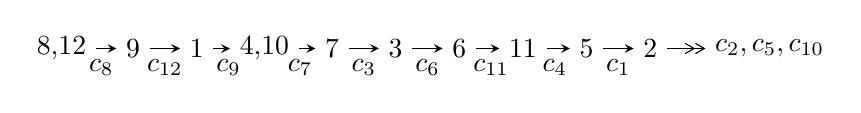
\begin{tikzpicture}[x=23pt, y=7pt]
	% node
	\node (A0) at (-1/8, 0) {8,12};
	\node (A1) at (1, 0) {9};
	\node (A2) at (2, 0) {1};
	\node (A3) at (49/16, 0) {4,10};
	\node (A4) at (33/8, 0) {7};
	\node (A5) at (41/8, 0) {3};
	\node (A6) at (49/8, 0) {6};
	\node (A7) at (57/8, 0) {11};
	\node (A8) at (65/8, 0) {5};
	\node (A9) at (73/8, 0) {2};
	\node (C1) at (1/2, -1) {$c_{8}$};
	\node (C2) at (3/2, -1) {$c_{12}$};
	\node (C3) at (5/2, -1) {$c_{9}$};
	\node (C4) at (29/8, -1) {$c_{7}$};
	\node (C5) at (37/8, -1) {$c_{3}$};
	\node (C6) at (45/8, -1) {$c_{6}$};
	\node (C7) at (53/8, -1) {$c_{11}$};
	\node (C8) at (61/8, -1) {$c_{4}$};
	\node (C9) at (69/8, -1) {$c_{1}$};
	\node (A10) at (11, 0) {$c_{2},c_{5},c_{10}$};

	% edge
	\draw[->,>=stealth]	
	(A0) edge (A1) (A1) edge (A2) (A2) edge (A3) (A3) edge (A4) (A4) edge (A5) (A5) edge (A6) (A6) edge (A7) (A7) edge (A8) (A8) edge (A9) ;
	\draw[->>,>={angle 60}]	
	(A9) edge (A10);
\end{tikzpicture} \\ 

\end{tabular} \\

\footnotetext{
The image of knot diagram is generated by the software ``\textbf{Draw programme}" developed by Andrew Bartholomew(\url{http://www.layer8.co.uk/maths/draw/index.htm\#Running-draw}), where we modified some parts for our purpose(\url{https://github.com/CATsTAILs/LinksPainter}).
}\phantom \\ \newline 
\centering \textbf{Ideals for irreducible components\footnotemark of $X_{\text{par}}$} 
 
\begin{align*}
I^u_{1}&=\langle 
8.75661\times10^{64} u^{63}+2.76997\times10^{65} u^{62}+\cdots+1.65696\times10^{65} b+2.96457\times10^{65},\\
\phantom{I^u_{1}}&\phantom{= \langle  }1.00296\times10^{66} u^{63}+3.44551\times10^{66} u^{62}+\cdots+8.28478\times10^{64} a+2.84103\times10^{65},\;u^{64}+4 u^{63}+\cdots-10 u+1\rangle \\
I^u_{2}&=\langle 
b-1,\;a+2,\;u+1\rangle \\
I^u_{3}&=\langle 
b+1,\;a^2-4 a+2,\;u+1\rangle \\
\\
\end{align*}
\raggedright * 3 irreducible components of $\dim_{\mathbb{C}}=0$, with total 67 representations.\\
\footnotetext{All coefficients of polynomials are rational numbers. But the coefficients are sometimes approximated in decimal forms when there is not enough margin.}
\newpage
\renewcommand{\arraystretch}{1}
\centering \section*{I. $I^u_{1}= \langle 8.76\times10^{64} u^{63}+2.77\times10^{65} u^{62}+\cdots+1.66\times10^{65} b+2.96\times10^{65},\;1.00\times10^{66} u^{63}+3.45\times10^{66} u^{62}+\cdots+8.28\times10^{64} a+2.84\times10^{65},\;u^{64}+4 u^{63}+\cdots-10 u+1 \rangle$}
\flushleft \textbf{(i) Arc colorings}\\
\begin{tabular}{m{7pt} m{180pt} m{7pt} m{180pt} }
\flushright $a_{8}=$&$\begin{pmatrix}1\\0\end{pmatrix}$ \\
\flushright $a_{12}=$&$\begin{pmatrix}0\\u\end{pmatrix}$ \\
\flushright $a_{9}=$&$\begin{pmatrix}1\\- u^2\end{pmatrix}$ \\
\flushright $a_{1}=$&$\begin{pmatrix}u\\- u^3+u\end{pmatrix}$ \\
\flushright $a_{4}=$&$\begin{pmatrix}-12.1060 u^{63}-41.5885 u^{62}+\cdots+205.872 u-3.42922\\-0.528476 u^{63}-1.67172 u^{62}+\cdots+7.65402 u-1.78916\end{pmatrix}$ \\
\flushright $a_{10}=$&$\begin{pmatrix}- u^2+1\\u^4-2 u^2\end{pmatrix}$ \\
\flushright $a_{7}=$&$\begin{pmatrix}13.7729 u^{63}+46.8393 u^{62}+\cdots-229.931 u+4.46101\\0.181537 u^{63}+0.533529 u^{62}+\cdots-1.36851 u+1.37956\end{pmatrix}$ \\
\flushright $a_{3}=$&$\begin{pmatrix}4.35303 u^{63}+10.6700 u^{62}+\cdots-32.5922 u-0.381251\\-3.47471 u^{63}-8.31368 u^{62}+\cdots+28.6251 u-2.38908\end{pmatrix}$ \\
\flushright $a_{6}=$&$\begin{pmatrix}8.57909 u^{63}+30.0107 u^{62}+\cdots-140.536 u-4.30529\\5.95601 u^{63}+19.1387 u^{62}+\cdots-97.4281 u+9.72466\end{pmatrix}$ \\
\flushright $a_{11}=$&$\begin{pmatrix}- u\\u\end{pmatrix}$ \\
\flushright $a_{5}=$&$\begin{pmatrix}-7.27418 u^{63}-25.7859 u^{62}+\cdots+120.459 u+3.84863\\-5.36032 u^{63}-17.4743 u^{62}+\cdots+93.0670 u-9.06702\end{pmatrix}$ \\
\flushright $a_{2}=$&$\begin{pmatrix}-8.95289 u^{63}-28.0262 u^{62}+\cdots+182.432 u-36.5824\\-5.59890 u^{63}-20.4560 u^{62}+\cdots+122.657 u-8.92048\end{pmatrix}$\\&\end{tabular}
\flushleft \textbf{(ii) Obstruction class $= -1$}\\~\\
\flushleft \textbf{(iii) Cusp Shapes $= -112.789 u^{63}-383.132 u^{62}+\cdots+2107.64 u-184.302$}\\~\\
\newpage\renewcommand{\arraystretch}{1}
\flushleft \textbf{(iv) u-Polynomials at the component}\newline \\
\begin{tabular}{m{50pt}|m{274pt}}
Crossings & \hspace{64pt}u-Polynomials at each crossing \\
\hline $$\begin{aligned}c_{1},c_{2},c_{5}\end{aligned}$$&$\begin{aligned}
&u^{64}+5 u^{63}+\cdots-6 u-2
\end{aligned}$\\
\hline $$\begin{aligned}c_{3},c_{7}\end{aligned}$$&$\begin{aligned}
&u^{64}-2 u^{63}+\cdots+6 u-1
\end{aligned}$\\
\hline $$\begin{aligned}c_{4}\end{aligned}$$&$\begin{aligned}
&u^{64}+16 u^{63}+\cdots-397046 u+45841
\end{aligned}$\\
\hline $$\begin{aligned}c_{6}\end{aligned}$$&$\begin{aligned}
&u^{64}-18 u^{63}+\cdots-8 u+1
\end{aligned}$\\
\hline $$\begin{aligned}c_{8},c_{9},c_{11}\\c_{12}\end{aligned}$$&$\begin{aligned}
&u^{64}-4 u^{63}+\cdots+10 u+1
\end{aligned}$\\
\hline $$\begin{aligned}c_{10}\end{aligned}$$&$\begin{aligned}
&u^{64}-2 u^{63}+\cdots-2 u-1
\end{aligned}$\\
\hline
\end{tabular}\\~\\
\newpage\renewcommand{\arraystretch}{1}
\flushleft \textbf{(v) Riley Polynomials at the component}\newline \\
\begin{tabular}{m{50pt}|m{274pt}}
Crossings & \hspace{64pt}Riley Polynomials at each crossing \\
\hline $$\begin{aligned}c_{1},c_{2},c_{5}\end{aligned}$$&$\begin{aligned}
&y^{64}-61 y^{63}+\cdots+12 y+4
\end{aligned}$\\
\hline $$\begin{aligned}c_{3},c_{7}\end{aligned}$$&$\begin{aligned}
&y^{64}-52 y^{63}+\cdots+6 y+1
\end{aligned}$\\
\hline $$\begin{aligned}c_{4}\end{aligned}$$&$\begin{aligned}
&y^{64}-440 y^{63}+\cdots+63549675954 y+2101397281
\end{aligned}$\\
\hline $$\begin{aligned}c_{6}\end{aligned}$$&$\begin{aligned}
&y^{64}-504 y^{63}+\cdots-638 y+1
\end{aligned}$\\
\hline $$\begin{aligned}c_{8},c_{9},c_{11}\\c_{12}\end{aligned}$$&$\begin{aligned}
&y^{64}-76 y^{63}+\cdots-106 y+1
\end{aligned}$\\
\hline $$\begin{aligned}c_{10}\end{aligned}$$&$\begin{aligned}
&y^{64}-8 y^{63}+\cdots-114 y+1
\end{aligned}$\\
\hline
\end{tabular}\\~\\
\newpage\flushleft \textbf{(vi) Complex Volumes and Cusp Shapes}
$$\begin{array}{c|c|c}  
\text{Solutions to }I^u_{1}& \I (\text{vol} + \sqrt{-1}CS) & \text{Cusp shape}\\
 \hline 
\begin{aligned}
u &= -0.626252 + 0.772749 I \\
a &= -0.442645 - 0.836072 I \\
b &= \phantom{-}1.282870 - 0.069070 I\end{aligned}
 & \phantom{-}1.37703 - 2.62298 I & \phantom{-0.000000 } 0 \\ \hline\begin{aligned}
u &= -0.626252 - 0.772749 I \\
a &= -0.442645 + 0.836072 I \\
b &= \phantom{-}1.282870 + 0.069070 I\end{aligned}
 & \phantom{-}1.37703 + 2.62298 I & \phantom{-0.000000 } 0 \\ \hline\begin{aligned}
u &= \phantom{-}0.892186 + 0.475186 I \\
a &= \phantom{-}1.45927 - 1.01010 I \\
b &= -1.37477 - 0.41692 I\end{aligned}
 & \phantom{-}5.33163 + 8.09564 I & \phantom{-0.000000 } 0 \\ \hline\begin{aligned}
u &= \phantom{-}0.892186 - 0.475186 I \\
a &= \phantom{-}1.45927 + 1.01010 I \\
b &= -1.37477 + 0.41692 I\end{aligned}
 & \phantom{-}5.33163 - 8.09564 I & \phantom{-0.000000 } 0 \\ \hline\begin{aligned}
u &= -0.885933 + 0.573263 I \\
a &= \phantom{-}0.924110 + 0.935341 I \\
b &= -1.224840 - 0.045601 I\end{aligned}
 & \phantom{-}4.82419 - 0.31393 I & \phantom{-0.000000 } 0 \\ \hline\begin{aligned}
u &= -0.885933 - 0.573263 I \\
a &= \phantom{-}0.924110 - 0.935341 I \\
b &= -1.224840 + 0.045601 I\end{aligned}
 & \phantom{-}4.82419 + 0.31393 I & \phantom{-0.000000 } 0 \\ \hline\begin{aligned}
u &= \phantom{-}0.866924 + 0.614790 I \\
a &= -1.33885 + 1.11410 I \\
b &= \phantom{-}1.36865 + 0.42563 I\end{aligned}
 & -0.85685 + 11.92020 I & \phantom{-0.000000 } 0 \\ \hline\begin{aligned}
u &= \phantom{-}0.866924 - 0.614790 I \\
a &= -1.33885 - 1.11410 I \\
b &= \phantom{-}1.36865 - 0.42563 I\end{aligned}
 & -0.85685 - 11.92020 I & \phantom{-0.000000 } 0 \\ \hline\begin{aligned}
u &= -1.088320 + 0.183319 I \\
a &= -1.033310 + 0.040437 I \\
b &= \phantom{-}0.007127 - 0.240948 I\end{aligned}
 & -3.32236 + 0.09828 I & \phantom{-0.000000 } 0 \\ \hline\begin{aligned}
u &= -1.088320 - 0.183319 I \\
a &= -1.033310 - 0.040437 I \\
b &= \phantom{-}0.007127 + 0.240948 I\end{aligned}
 & -3.32236 - 0.09828 I & \phantom{-0.000000 } 0\\
 \hline 
 \end{array}$$\newpage$$\begin{array}{c|c|c}  
\text{Solutions to }I^u_{1}& \I (\text{vol} + \sqrt{-1}CS) & \text{Cusp shape}\\
 \hline 
\begin{aligned}
u &= \phantom{-}0.727414 + 0.497209 I \\
a &= \phantom{-}0.517608 - 0.186664 I \\
b &= -0.136718 - 0.955922 I\end{aligned}
 & -5.57662 + 7.00157 I & \phantom{-0.000000 } 0 \\ \hline\begin{aligned}
u &= \phantom{-}0.727414 - 0.497209 I \\
a &= \phantom{-}0.517608 + 0.186664 I \\
b &= -0.136718 + 0.955922 I\end{aligned}
 & -5.57662 - 7.00157 I & \phantom{-0.000000 } 0 \\ \hline\begin{aligned}
u &= \phantom{-}0.086190 + 0.869107 I \\
a &= -0.161462 - 0.186514 I \\
b &= \phantom{-}1.276990 - 0.329837 I\end{aligned}
 & -3.24005 - 7.03352 I & \phantom{-0.000000 } 0 \\ \hline\begin{aligned}
u &= \phantom{-}0.086190 - 0.869107 I \\
a &= -0.161462 + 0.186514 I \\
b &= \phantom{-}1.276990 + 0.329837 I\end{aligned}
 & -3.24005 + 7.03352 I & \phantom{-0.000000 } 0 \\ \hline\begin{aligned}
u &= \phantom{-}0.826064 + 0.274343 I \\
a &= -1.68330 + 0.81928 I \\
b &= \phantom{-}1.39853 + 0.42614 I\end{aligned}
 & \phantom{-}4.75434 + 3.17966 I & \phantom{-0.000000 } 0 \\ \hline\begin{aligned}
u &= \phantom{-}0.826064 - 0.274343 I \\
a &= -1.68330 - 0.81928 I \\
b &= \phantom{-}1.39853 - 0.42614 I\end{aligned}
 & \phantom{-}4.75434 - 3.17966 I & \phantom{-0.000000 } 0 \\ \hline\begin{aligned}
u &= -1.20392\phantom{ +0.000000I} \\
a &= \phantom{-}1.35869\phantom{ +0.000000I} \\
b &= -0.745445\phantom{ +0.000000I}\end{aligned}
 & \phantom{-}2.67121\phantom{ +0.000000I} & \phantom{-0.000000 } 0 \\ \hline\begin{aligned}
u &= -0.735824\phantom{ +0.000000I} \\
a &= -4.70570\phantom{ +0.000000I} \\
b &= \phantom{-}1.05067\phantom{ +0.000000I}\end{aligned}
 & \phantom{-}2.92949\phantom{ +0.000000I} & -31.0790\phantom{ +0.000000I} \\ \hline\begin{aligned}
u &= -0.061375 + 0.731517 I \\
a &= -0.056369 + 0.272785 I \\
b &= -1.230620 + 0.271880 I\end{aligned}
 & \phantom{-}2.42658 - 4.10040 I & \phantom{-}5.18854 + 6.65155 I \\ \hline\begin{aligned}
u &= -0.061375 - 0.731517 I \\
a &= -0.056369 - 0.272785 I \\
b &= -1.230620 - 0.271880 I\end{aligned}
 & \phantom{-}2.42658 + 4.10040 I & \phantom{-}5.18854 - 6.65155 I\\
 \hline 
 \end{array}$$\newpage$$\begin{array}{c|c|c}  
\text{Solutions to }I^u_{1}& \I (\text{vol} + \sqrt{-1}CS) & \text{Cusp shape}\\
 \hline 
\begin{aligned}
u &= -1.156350 + 0.575363 I \\
a &= -1.056810 - 0.610432 I \\
b &= \phantom{-}1.251050 + 0.169381 I\end{aligned}
 & \phantom{-}0.45977 + 2.04940 I & \phantom{-0.000000 } 0 \\ \hline\begin{aligned}
u &= -1.156350 - 0.575363 I \\
a &= -1.056810 + 0.610432 I \\
b &= \phantom{-}1.251050 - 0.169381 I\end{aligned}
 & \phantom{-}0.45977 - 2.04940 I & \phantom{-0.000000 } 0 \\ \hline\begin{aligned}
u &= \phantom{-}0.645610 + 0.280609 I \\
a &= -0.622762 - 0.084173 I \\
b &= \phantom{-}0.227169 + 0.986896 I\end{aligned}
 & \phantom{-}0.39947 + 3.16035 I & \phantom{-}2.81338 - 10.76378 I \\ \hline\begin{aligned}
u &= \phantom{-}0.645610 - 0.280609 I \\
a &= -0.622762 + 0.084173 I \\
b &= \phantom{-}0.227169 - 0.986896 I\end{aligned}
 & \phantom{-}0.39947 - 3.16035 I & \phantom{-}2.81338 + 10.76378 I \\ \hline\begin{aligned}
u &= -0.537409 + 0.416579 I \\
a &= -0.908169 + 1.049400 I \\
b &= -0.301281 + 0.283446 I\end{aligned}
 & -3.30500 - 1.49850 I & -1.71841 + 4.52498 I \\ \hline\begin{aligned}
u &= -0.537409 - 0.416579 I \\
a &= -0.908169 - 1.049400 I \\
b &= -0.301281 - 0.283446 I\end{aligned}
 & -3.30500 + 1.49850 I & -1.71841 - 4.52498 I \\ \hline\begin{aligned}
u &= \phantom{-}0.171438 + 0.641396 I \\
a &= -0.810739 + 0.661600 I \\
b &= -0.011504 + 0.735189 I\end{aligned}
 & -7.24617 - 3.15234 I & -4.81813 + 1.66839 I \\ \hline\begin{aligned}
u &= \phantom{-}0.171438 - 0.641396 I \\
a &= -0.810739 - 0.661600 I \\
b &= -0.011504 - 0.735189 I\end{aligned}
 & -7.24617 + 3.15234 I & -4.81813 - 1.66839 I \\ \hline\begin{aligned}
u &= -0.622251 + 0.147718 I \\
a &= \phantom{-}0.623442 - 0.530311 I \\
b &= \phantom{-}0.140050 - 0.093500 I\end{aligned}
 & \phantom{-}1.153010 - 0.371044 I & \phantom{-}8.52101 + 0.53269 I \\ \hline\begin{aligned}
u &= -0.622251 - 0.147718 I \\
a &= \phantom{-}0.623442 + 0.530311 I \\
b &= \phantom{-}0.140050 + 0.093500 I\end{aligned}
 & \phantom{-}1.153010 + 0.371044 I & \phantom{-}8.52101 - 0.53269 I\\
 \hline 
 \end{array}$$\newpage$$\begin{array}{c|c|c}  
\text{Solutions to }I^u_{1}& \I (\text{vol} + \sqrt{-1}CS) & \text{Cusp shape}\\
 \hline 
\begin{aligned}
u &= -0.625236\phantom{ +0.000000I} \\
a &= -32.6722\phantom{ +0.000000I} \\
b &= -0.982597\phantom{ +0.000000I}\end{aligned}
 & -2.29108\phantom{ +0.000000I} & -335.850\phantom{ +0.000000I} \\ \hline\begin{aligned}
u &= \phantom{-}0.571354 + 0.216286 I \\
a &= \phantom{-}1.058770 - 0.384713 I \\
b &= -1.136650 + 0.669884 I\end{aligned}
 & -2.52737 + 1.49035 I & -1.46490 - 10.14674 I \\ \hline\begin{aligned}
u &= \phantom{-}0.571354 - 0.216286 I \\
a &= \phantom{-}1.058770 + 0.384713 I \\
b &= -1.136650 - 0.669884 I\end{aligned}
 & -2.52737 - 1.49035 I & -1.46490 + 10.14674 I \\ \hline\begin{aligned}
u &= -1.58313\phantom{ +0.000000I} \\
a &= \phantom{-}2.77393\phantom{ +0.000000I} \\
b &= -1.86821\phantom{ +0.000000I}\end{aligned}
 & \phantom{-}3.83757\phantom{ +0.000000I} & \phantom{-0.000000 } 0 \\ \hline\begin{aligned}
u &= \phantom{-}1.58050 + 0.10884 I \\
a &= \phantom{-}0.006317 - 0.340356 I \\
b &= -0.242493 - 0.631350 I\end{aligned}
 & \phantom{-}3.96868 + 3.34904 I & \phantom{-0.000000 } 0 \\ \hline\begin{aligned}
u &= \phantom{-}1.58050 - 0.10884 I \\
a &= \phantom{-}0.006317 + 0.340356 I \\
b &= -0.242493 + 0.631350 I\end{aligned}
 & \phantom{-}3.96868 - 3.34904 I & \phantom{-0.000000 } 0 \\ \hline\begin{aligned}
u &= -1.58979 + 0.03598 I \\
a &= \phantom{-}1.41098 + 0.68557 I \\
b &= -1.17421 - 1.06495 I\end{aligned}
 & \phantom{-}4.95069 - 2.27479 I & \phantom{-0.000000 } 0 \\ \hline\begin{aligned}
u &= -1.58979 - 0.03598 I \\
a &= \phantom{-}1.41098 - 0.68557 I \\
b &= -1.17421 + 1.06495 I\end{aligned}
 & \phantom{-}4.95069 + 2.27479 I & \phantom{-0.000000 } 0 \\ \hline\begin{aligned}
u &= -1.60546 + 0.05832 I \\
a &= -0.671440 + 0.764979 I \\
b &= \phantom{-}0.437967 - 1.302070 I\end{aligned}
 & \phantom{-}8.17400 - 4.30296 I & \phantom{-0.000000 } 0 \\ \hline\begin{aligned}
u &= -1.60546 - 0.05832 I \\
a &= -0.671440 - 0.764979 I \\
b &= \phantom{-}0.437967 + 1.302070 I\end{aligned}
 & \phantom{-}8.17400 + 4.30296 I & \phantom{-0.000000 } 0\\
 \hline 
 \end{array}$$\newpage$$\begin{array}{c|c|c}  
\text{Solutions to }I^u_{1}& \I (\text{vol} + \sqrt{-1}CS) & \text{Cusp shape}\\
 \hline 
\begin{aligned}
u &= \phantom{-}1.60877 + 0.03569 I \\
a &= \phantom{-}0.077213 + 0.292537 I \\
b &= \phantom{-}0.219375 + 0.411958 I\end{aligned}
 & \phantom{-}8.93615 + 1.02069 I & \phantom{-0.000000 } 0 \\ \hline\begin{aligned}
u &= \phantom{-}1.60877 - 0.03569 I \\
a &= \phantom{-}0.077213 - 0.292537 I \\
b &= \phantom{-}0.219375 - 0.411958 I\end{aligned}
 & \phantom{-}8.93615 - 1.02069 I & \phantom{-0.000000 } 0 \\ \hline\begin{aligned}
u &= \phantom{-}0.385731\phantom{ +0.000000I} \\
a &= \phantom{-}4.06256\phantom{ +0.000000I} \\
b &= -1.41196\phantom{ +0.000000I}\end{aligned}
 & -3.33490\phantom{ +0.000000I} & -8.92110\phantom{ +0.000000I} \\ \hline\begin{aligned}
u &= \phantom{-}0.129453 + 0.356601 I \\
a &= \phantom{-}1.25594 - 0.67953 I \\
b &= -0.129998 - 0.580705 I\end{aligned}
 & -1.019940 - 0.841014 I & -4.44164 + 2.44385 I \\ \hline\begin{aligned}
u &= \phantom{-}0.129453 - 0.356601 I \\
a &= \phantom{-}1.25594 + 0.67953 I \\
b &= -0.129998 + 0.580705 I\end{aligned}
 & -1.019940 + 0.841014 I & -4.44164 - 2.44385 I \\ \hline\begin{aligned}
u &= -0.151171 + 0.347893 I \\
a &= \phantom{-}1.51053 - 0.33569 I \\
b &= \phantom{-}1.087870 - 0.202838 I\end{aligned}
 & \phantom{-}1.93096 - 1.01785 I & \phantom{-}2.25227 - 1.57609 I \\ \hline\begin{aligned}
u &= -0.151171 - 0.347893 I \\
a &= \phantom{-}1.51053 + 0.33569 I \\
b &= \phantom{-}1.087870 + 0.202838 I\end{aligned}
 & \phantom{-}1.93096 + 1.01785 I & \phantom{-}2.25227 + 1.57609 I \\ \hline\begin{aligned}
u &= -1.61625 + 0.13512 I \\
a &= \phantom{-}0.579253 - 0.473421 I \\
b &= -0.254582 + 1.128060 I\end{aligned}
 & \phantom{-}2.39807 - 9.34049 I & \phantom{-0.000000 } 0 \\ \hline\begin{aligned}
u &= -1.61625 - 0.13512 I \\
a &= \phantom{-}0.579253 + 0.473421 I \\
b &= -0.254582 - 1.128060 I\end{aligned}
 & \phantom{-}2.39807 + 9.34049 I & \phantom{-0.000000 } 0 \\ \hline\begin{aligned}
u &= \phantom{-}1.63116 + 0.01107 I \\
a &= -1.17537 + 1.13475 I \\
b &= -0.795270 + 0.143585 I\end{aligned}
 & \phantom{-}5.71807 + 0.01867 I & \phantom{-0.000000 } 0\\
 \hline 
 \end{array}$$\newpage$$\begin{array}{c|c|c}  
\text{Solutions to }I^u_{1}& \I (\text{vol} + \sqrt{-1}CS) & \text{Cusp shape}\\
 \hline 
\begin{aligned}
u &= \phantom{-}1.63116 - 0.01107 I \\
a &= -1.17537 - 1.13475 I \\
b &= -0.795270 - 0.143585 I\end{aligned}
 & \phantom{-}5.71807 - 0.01867 I & \phantom{-0.000000 } 0 \\ \hline\begin{aligned}
u &= \phantom{-}1.62771 + 0.23629 I \\
a &= -1.53783 + 0.68857 I \\
b &= \phantom{-}1.350810 + 0.224077 I\end{aligned}
 & \phantom{-}8.99118 + 6.39006 I & \phantom{-0.000000 } 0 \\ \hline\begin{aligned}
u &= \phantom{-}1.62771 - 0.23629 I \\
a &= -1.53783 - 0.68857 I \\
b &= \phantom{-}1.350810 - 0.224077 I\end{aligned}
 & \phantom{-}8.99118 - 6.39006 I & \phantom{-0.000000 } 0 \\ \hline\begin{aligned}
u &= -1.65093 + 0.07673 I \\
a &= -2.22460 - 0.22306 I \\
b &= \phantom{-}1.61684 - 0.49505 I\end{aligned}
 & \phantom{-}13.36180 - 4.53477 I & \phantom{-0.000000 } 0 \\ \hline\begin{aligned}
u &= -1.65093 - 0.07673 I \\
a &= -2.22460 + 0.22306 I \\
b &= \phantom{-}1.61684 + 0.49505 I\end{aligned}
 & \phantom{-}13.36180 + 4.53477 I & \phantom{-0.000000 } 0 \\ \hline\begin{aligned}
u &= -1.67065 + 0.13316 I \\
a &= \phantom{-}2.09031 + 0.47257 I \\
b &= -1.51390 + 0.48815 I\end{aligned}
 & \phantom{-}14.1665 - 10.4624 I & \phantom{-0.000000 } 0 \\ \hline\begin{aligned}
u &= -1.67065 - 0.13316 I \\
a &= \phantom{-}2.09031 - 0.47257 I \\
b &= -1.51390 - 0.48815 I\end{aligned}
 & \phantom{-}14.1665 + 10.4624 I & \phantom{-0.000000 } 0 \\ \hline\begin{aligned}
u &= -1.66778 + 0.18149 I \\
a &= -2.03991 - 0.65692 I \\
b &= \phantom{-}1.46024 - 0.47787 I\end{aligned}
 & \phantom{-}7.7777 - 15.0108 I & \phantom{-0.000000 } 0 \\ \hline\begin{aligned}
u &= -1.66778 - 0.18149 I \\
a &= -2.03991 + 0.65692 I \\
b &= \phantom{-}1.46024 + 0.47787 I\end{aligned}
 & \phantom{-}7.7777 + 15.0108 I & \phantom{-0.000000 } 0 \\ \hline\begin{aligned}
u &= \phantom{-}1.68055\phantom{ +0.000000I} \\
a &= -2.49868\phantom{ +0.000000I} \\
b &= \phantom{-}1.25013\phantom{ +0.000000I}\end{aligned}
 & \phantom{-}11.5859\phantom{ +0.000000I} & \phantom{-0.000000 } 0\\
 \hline 
 \end{array}$$\newpage$$\begin{array}{c|c|c}  
\text{Solutions to }I^u_{1}& \I (\text{vol} + \sqrt{-1}CS) & \text{Cusp shape}\\
 \hline 
\begin{aligned}
u &= \phantom{-}1.68516 + 0.14611 I \\
a &= \phantom{-}1.76330 - 0.59949 I \\
b &= -1.328680 - 0.151173 I\end{aligned}
 & \phantom{-}13.75650 + 3.08420 I & \phantom{-0.000000 } 0 \\ \hline\begin{aligned}
u &= \phantom{-}1.68516 - 0.14611 I \\
a &= \phantom{-}1.76330 + 0.59949 I \\
b &= -1.328680 + 0.151173 I\end{aligned}
 & \phantom{-}13.75650 - 3.08420 I & \phantom{-0.000000 } 0 \\ \hline\begin{aligned}
u &= \phantom{-}1.73966\phantom{ +0.000000I} \\
a &= -2.03600\phantom{ +0.000000I} \\
b &= \phantom{-}1.32403\phantom{ +0.000000I}\end{aligned}
 & \phantom{-}11.5124\phantom{ +0.000000I} & \phantom{-0.000000 } 0 \\ \hline\begin{aligned}
u &= \phantom{-}0.102209\phantom{ +0.000000I} \\
a &= \phantom{-}13.6904\phantom{ +0.000000I} \\
b &= -1.15668\phantom{ +0.000000I}\end{aligned}
 & -3.39768\phantom{ +0.000000I} & -3.12270\phantom{ +0.000000I}\\
 \hline 
 \end{array}$$\newpage\newpage\renewcommand{\arraystretch}{1}
\centering \section*{II. $I^u_{2}= \langle b-1,\;a+2,\;u+1 \rangle$}
\flushleft \textbf{(i) Arc colorings}\\
\begin{tabular}{m{7pt} m{180pt} m{7pt} m{180pt} }
\flushright $a_{8}=$&$\begin{pmatrix}1\\0\end{pmatrix}$ \\
\flushright $a_{12}=$&$\begin{pmatrix}0\\-1\end{pmatrix}$ \\
\flushright $a_{9}=$&$\begin{pmatrix}1\\-1\end{pmatrix}$ \\
\flushright $a_{1}=$&$\begin{pmatrix}-1\\0\end{pmatrix}$ \\
\flushright $a_{4}=$&$\begin{pmatrix}-2\\1\end{pmatrix}$ \\
\flushright $a_{10}=$&$\begin{pmatrix}0\\-1\end{pmatrix}$ \\
\flushright $a_{7}=$&$\begin{pmatrix}-1\\1\end{pmatrix}$ \\
\flushright $a_{3}=$&$\begin{pmatrix}-1\\0\end{pmatrix}$ \\
\flushright $a_{6}=$&$\begin{pmatrix}-1\\0\end{pmatrix}$ \\
\flushright $a_{11}=$&$\begin{pmatrix}1\\-1\end{pmatrix}$ \\
\flushright $a_{5}=$&$\begin{pmatrix}-1\\0\end{pmatrix}$ \\
\flushright $a_{2}=$&$\begin{pmatrix}-1\\0\end{pmatrix}$\\&\end{tabular}
\flushleft \textbf{(ii) Obstruction class $= 1$}\\~\\
\flushleft \textbf{(iii) Cusp Shapes $= 12$}\\~\\
\newpage\renewcommand{\arraystretch}{1}
\flushleft \textbf{(iv) u-Polynomials at the component}\newline \\
\begin{tabular}{m{50pt}|m{274pt}}
Crossings & \hspace{64pt}u-Polynomials at each crossing \\
\hline $$\begin{aligned}c_{1},c_{2},c_{5}\end{aligned}$$&$\begin{aligned}
&u
\end{aligned}$\\
\hline $$\begin{aligned}c_{3},c_{8},c_{9}\\c_{10}\end{aligned}$$&$\begin{aligned}
&u+1
\end{aligned}$\\
\hline $$\begin{aligned}c_{4},c_{6},c_{7}\\c_{11},c_{12}\end{aligned}$$&$\begin{aligned}
&u-1
\end{aligned}$\\
\hline
\end{tabular}\\~\\
\newpage\renewcommand{\arraystretch}{1}
\flushleft \textbf{(v) Riley Polynomials at the component}\newline \\
\begin{tabular}{m{50pt}|m{274pt}}
Crossings & \hspace{64pt}Riley Polynomials at each crossing \\
\hline $$\begin{aligned}c_{1},c_{2},c_{5}\end{aligned}$$&$\begin{aligned}
&y
\end{aligned}$\\
\hline $$\begin{aligned}c_{3},c_{4},c_{6}\\c_{7},c_{8},c_{9}\\c_{10},c_{11},c_{12}\end{aligned}$$&$\begin{aligned}
&y-1
\end{aligned}$\\
\hline
\end{tabular}\\~\\
\newpage\flushleft \textbf{(vi) Complex Volumes and Cusp Shapes}
$$\begin{array}{c|c|c}  
\text{Solutions to }I^u_{2}& \I (\text{vol} + \sqrt{-1}CS) & \text{Cusp shape}\\
 \hline 
\begin{aligned}
u &= -1.00000\phantom{ +0.000000I} \\
a &= -2.00000\phantom{ +0.000000I} \\
b &= \phantom{-}1.00000\phantom{ +0.000000I}\end{aligned}
 & \phantom{-}3.28987\phantom{ +0.000000I} & \phantom{-}12.0000\phantom{ +0.000000I}\\
 \hline 
 \end{array}$$\newpage\newpage\renewcommand{\arraystretch}{1}
\centering \section*{III. $I^u_{3}= \langle b+1,\;a^2-4 a+2,\;u+1 \rangle$}
\flushleft \textbf{(i) Arc colorings}\\
\begin{tabular}{m{7pt} m{180pt} m{7pt} m{180pt} }
\flushright $a_{8}=$&$\begin{pmatrix}1\\0\end{pmatrix}$ \\
\flushright $a_{12}=$&$\begin{pmatrix}0\\-1\end{pmatrix}$ \\
\flushright $a_{9}=$&$\begin{pmatrix}1\\-1\end{pmatrix}$ \\
\flushright $a_{1}=$&$\begin{pmatrix}-1\\0\end{pmatrix}$ \\
\flushright $a_{4}=$&$\begin{pmatrix}a\\-1\end{pmatrix}$ \\
\flushright $a_{10}=$&$\begin{pmatrix}0\\-1\end{pmatrix}$ \\
\flushright $a_{7}=$&$\begin{pmatrix}- a+1\\1\end{pmatrix}$ \\
\flushright $a_{3}=$&$\begin{pmatrix}1\\0\end{pmatrix}$ \\
\flushright $a_{6}=$&$\begin{pmatrix}- a+1\\- a+2\end{pmatrix}$ \\
\flushright $a_{11}=$&$\begin{pmatrix}1\\-1\end{pmatrix}$ \\
\flushright $a_{5}=$&$\begin{pmatrix}1\\a-2\end{pmatrix}$ \\
\flushright $a_{2}=$&$\begin{pmatrix}- a+1\\-2\end{pmatrix}$\\&\end{tabular}
\flushleft \textbf{(ii) Obstruction class $= 1$}\\~\\
\flushleft \textbf{(iii) Cusp Shapes $= 4$}\\~\\
\newpage\renewcommand{\arraystretch}{1}
\flushleft \textbf{(iv) u-Polynomials at the component}\newline \\
\begin{tabular}{m{50pt}|m{274pt}}
Crossings & \hspace{64pt}u-Polynomials at each crossing \\
\hline $$\begin{aligned}c_{1},c_{2},c_{5}\end{aligned}$$&$\begin{aligned}
&u^2-2
\end{aligned}$\\
\hline $$\begin{aligned}c_{3},c_{10},c_{11}\\c_{12}\end{aligned}$$&$\begin{aligned}
&(u-1)^2
\end{aligned}$\\
\hline $$\begin{aligned}c_{4}\end{aligned}$$&$\begin{aligned}
&u^2+2 u-1
\end{aligned}$\\
\hline $$\begin{aligned}c_{6}\end{aligned}$$&$\begin{aligned}
&u^2-2 u-1
\end{aligned}$\\
\hline $$\begin{aligned}c_{7},c_{8},c_{9}\end{aligned}$$&$\begin{aligned}
&(u+1)^2
\end{aligned}$\\
\hline
\end{tabular}\\~\\
\newpage\renewcommand{\arraystretch}{1}
\flushleft \textbf{(v) Riley Polynomials at the component}\newline \\
\begin{tabular}{m{50pt}|m{274pt}}
Crossings & \hspace{64pt}Riley Polynomials at each crossing \\
\hline $$\begin{aligned}c_{1},c_{2},c_{5}\end{aligned}$$&$\begin{aligned}
&(y-2)^2
\end{aligned}$\\
\hline $$\begin{aligned}c_{3},c_{7},c_{8}\\c_{9},c_{10},c_{11}\\c_{12}\end{aligned}$$&$\begin{aligned}
&(y-1)^2
\end{aligned}$\\
\hline $$\begin{aligned}c_{4},c_{6}\end{aligned}$$&$\begin{aligned}
&y^2-6 y+1
\end{aligned}$\\
\hline
\end{tabular}\\~\\
\newpage\flushleft \textbf{(vi) Complex Volumes and Cusp Shapes}
$$\begin{array}{c|c|c}  
\text{Solutions to }I^u_{3}& \I (\text{vol} + \sqrt{-1}CS) & \text{Cusp shape}\\
 \hline 
\begin{aligned}
u &= -1.00000\phantom{ +0.000000I} \\
a &= \phantom{-}0.585786\phantom{ +0.000000I} \\
b &= -1.00000\phantom{ +0.000000I}\end{aligned}
 & -1.64493\phantom{ +0.000000I} & \phantom{-}4.00000\phantom{ +0.000000I} \\ \hline\begin{aligned}
u &= -1.00000\phantom{ +0.000000I} \\
a &= \phantom{-}3.41421\phantom{ +0.000000I} \\
b &= -1.00000\phantom{ +0.000000I}\end{aligned}
 & -1.64493\phantom{ +0.000000I} & \phantom{-}4.00000\phantom{ +0.000000I}\\
 \hline 
 \end{array}$$\newpage
\newpage\renewcommand{\arraystretch}{1}
\centering \section*{ IV. u-Polynomials}
\begin{tabular}{m{50pt}|m{274pt}}
Crossings & \hspace{64pt}u-Polynomials at each crossing \\
\hline $$\begin{aligned}c_{1},c_{2},c_{5}\end{aligned}$$&$\begin{aligned}
&u(u^2-2)(u^{64}+5 u^{63}+\cdots-6 u-2)
\end{aligned}$\\
\hline $$\begin{aligned}c_{3}\end{aligned}$$&$\begin{aligned}
&((u-1)^2)(u+1)(u^{64}-2 u^{63}+\cdots+6 u-1)
\end{aligned}$\\
\hline $$\begin{aligned}c_{4}\end{aligned}$$&$\begin{aligned}
&(u-1)(u^2+2 u-1)(u^{64}+16 u^{63}+\cdots-397046 u+45841)
\end{aligned}$\\
\hline $$\begin{aligned}c_{6}\end{aligned}$$&$\begin{aligned}
&(u-1)(u^2-2 u-1)(u^{64}-18 u^{63}+\cdots-8 u+1)
\end{aligned}$\\
\hline $$\begin{aligned}c_{7}\end{aligned}$$&$\begin{aligned}
&(u-1)(u+1)^2(u^{64}-2 u^{63}+\cdots+6 u-1)
\end{aligned}$\\
\hline $$\begin{aligned}c_{8},c_{9}\end{aligned}$$&$\begin{aligned}
&((u+1)^3)(u^{64}-4 u^{63}+\cdots+10 u+1)
\end{aligned}$\\
\hline $$\begin{aligned}c_{10}\end{aligned}$$&$\begin{aligned}
&((u-1)^2)(u+1)(u^{64}-2 u^{63}+\cdots-2 u-1)
\end{aligned}$\\
\hline $$\begin{aligned}c_{11},c_{12}\end{aligned}$$&$\begin{aligned}
&((u-1)^3)(u^{64}-4 u^{63}+\cdots+10 u+1)
\end{aligned}$\\
\hline
\end{tabular}\newpage\renewcommand{\arraystretch}{1}
\centering \section*{ V. Riley Polynomials}
\begin{tabular}{m{50pt}|m{274pt}}
Crossings & \hspace{64pt}Riley Polynomials at each crossing \\
\hline $$\begin{aligned}c_{1},c_{2},c_{5}\end{aligned}$$&$\begin{aligned}
&y(y-2)^2(y^{64}-61 y^{63}+\cdots+12 y+4)
\end{aligned}$\\
\hline $$\begin{aligned}c_{3},c_{7}\end{aligned}$$&$\begin{aligned}
&((y-1)^3)(y^{64}-52 y^{63}+\cdots+6 y+1)
\end{aligned}$\\
\hline $$\begin{aligned}c_{4}\end{aligned}$$&$\begin{aligned}
&(y-1)(y^2-6 y+1)\\
&\cdot(y^{64}-440 y^{63}+\cdots+63549675954 y+2101397281)
\end{aligned}$\\
\hline $$\begin{aligned}c_{6}\end{aligned}$$&$\begin{aligned}
&(y-1)(y^2-6 y+1)(y^{64}-504 y^{63}+\cdots-638 y+1)
\end{aligned}$\\
\hline $$\begin{aligned}c_{8},c_{9},c_{11}\\c_{12}\end{aligned}$$&$\begin{aligned}
&((y-1)^3)(y^{64}-76 y^{63}+\cdots-106 y+1)
\end{aligned}$\\
\hline $$\begin{aligned}c_{10}\end{aligned}$$&$\begin{aligned}
&((y-1)^3)(y^{64}-8 y^{63}+\cdots-114 y+1)
\end{aligned}$\\
\hline
\end{tabular}
\vskip 2pc
\end{document}